\section{Lexikalanalys}

Eftersom det skulle skapas ett språk för att skanna \textit{fak.c}, valdes att enbart det alfabet
som \textit{fak.c} använder. Detta gjordes genom att titta på \textit{fak.c}.
\\ \textit{pas.l} användes som en mall för att utveckla språket för specifikt \textit{fak.c} 

\begin{figure}[!h]
    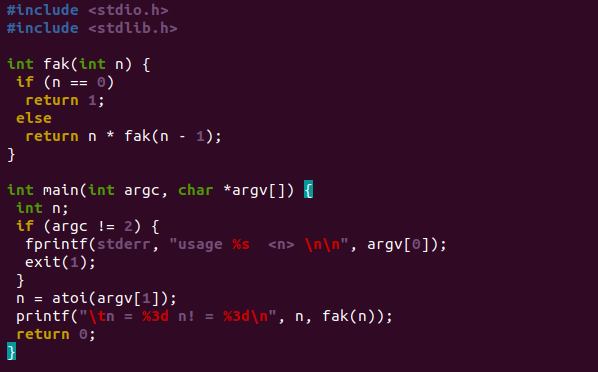
\includegraphics[width=\linewidth,height=3cm]{bilder/fak.c.png}
    \captionof{figure}{fak.c koden}
    \label{fig:fak.c}
\end{figure}

\\
\begin{figure}[!h]
    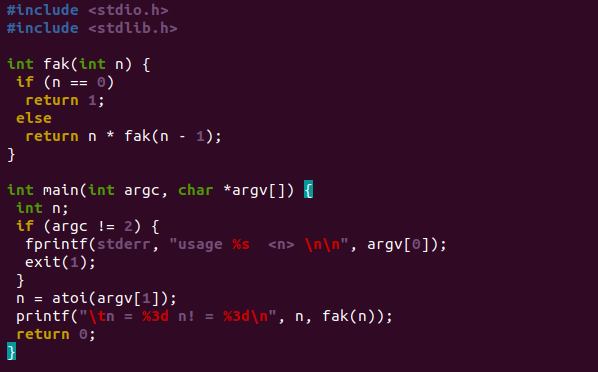
\includegraphics[width=\linewidth,height=3cm]{bilder/fak.c.png}
    \captionof{figure}{fak.l språket}
    \label{fig:fak.c}
\end{figure}

\\
\begin{description}

\item[\textit{#include}] I Figure[\ref{fig:fak.}] är \textit{#includ} ett token för importering av biblotek. 

\item[\textit{{ID}*.h} 
